%\let\textcircled=\pgftextcircled
\chapter{Input data cleaning}
\label{chap:input_data_cleaning}

Input data from sensors doesn't represent real measurement of vehicle physics quantities. Instruments have a measuring error, each one with different possible reasons. This chapter deals with techniques used in the project to reduce that error, whether it was experimental or systematic.

\section{Stationary time detection}
Most of the solutions used to remove errors are based on the assumption of a vehicle state, in particular the stationary one. \\
This can't be detected by a near zero acceleration along all axis because vehicle could be moving with constant speed. So integrated speed should be used, but integrating acceleration vectors that need corrections can bring next code logic to make mistakes as well as being a waste of time, because integration should be recalculated after having applied corrections. \\
One solution can be to use non-directional speed from GNSS data by the measure device in the box. But this speed is under effect of Kalman filters to avoid measurement errors The filter is implemented directly inside box firmware, but reacts late to changes. One can differentiate numerically the GNSS positions to get a more precise speed and, on top of that, calculate stationary times. The choice of using speed subject to Kalman filters or the one derived should be based on GNSS sensor precision. Especially when vehicle is stopped, its error can be relevant as showed in the following picture.
\begin{figure}[H]
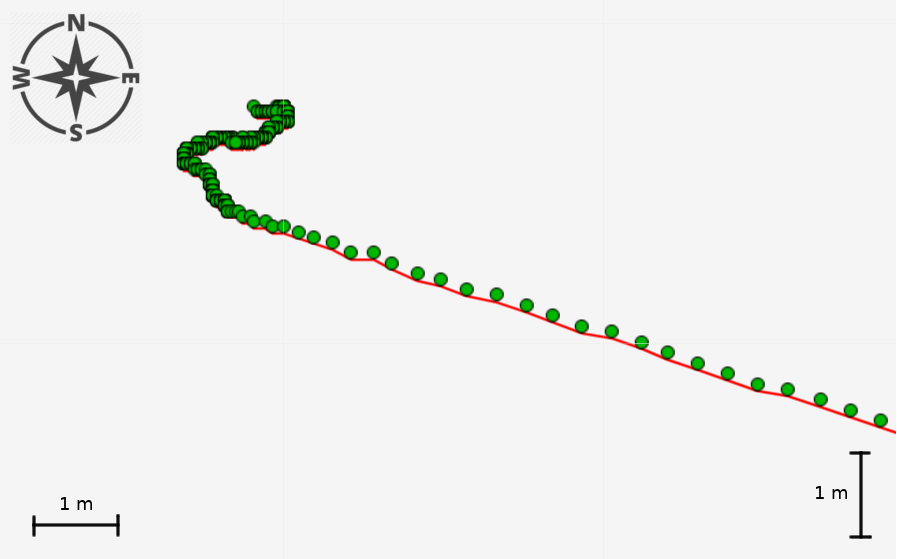
\includegraphics[width=\textwidth]{gnss_error_stationary_vehicle}
\caption{Green points represent GNSS positions. On top-left GNSS error can be noticed in a situation where vehicle was stopped during experiment}
\end{figure}
\justify
To try to handle input data where vehicle never really stops, the algorithm for stationary time detection searches into dataset with an increasing threshold, until enough periods are found.

\section{Gyroscope drift}
Gyroscopes have a drift and an offset that is unavoidable. \cite{6727722} \\
Offsets and their drift can be measured when vehicles are stationary. Average value of angular velocities in stationary moments is an approximation of gyroscope offset.
During motion, a gyroscope exposed to heat increase its drift. So I made sure drift removal was applied continuously at each stationary time, removing the drift detected onwards. 
\begin{figure}[H]
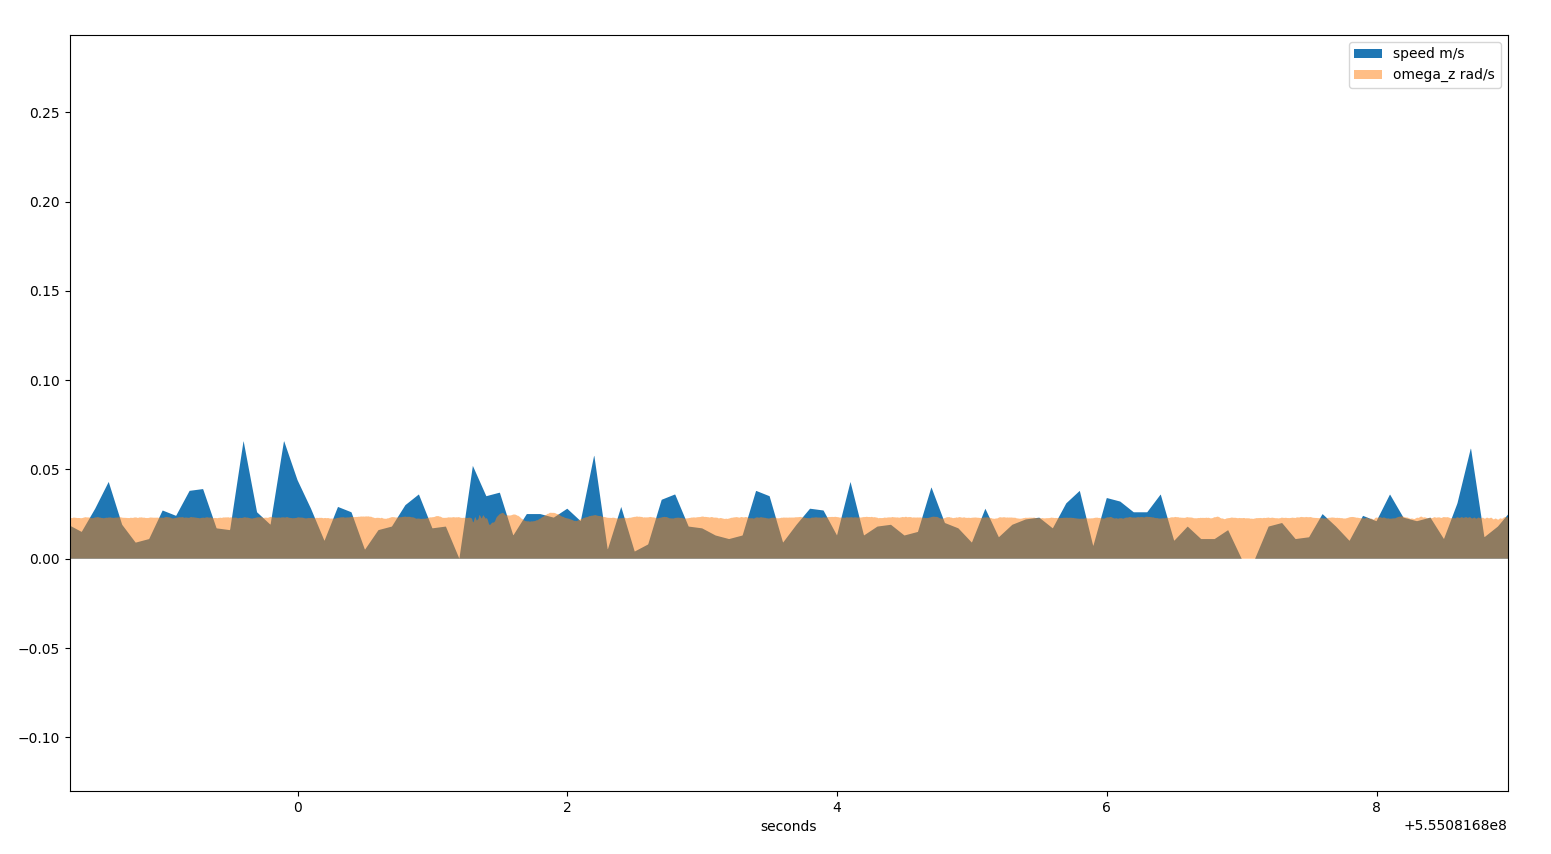
\includegraphics[width=\textwidth]{gyro_drift.png}
\caption{Data from stopped vehicle. Linear speed is near zero but gyroscope detects a non negligible angular speed}
\end{figure}

\section{Noise reduction}
Sensors are subject to noise both electronic (from the board itself or the electric supply) and mechanical (from their setup and the vehicle). In the data analyzed for this project I found spikes without any correlation to real events.
There are various techniques to remove them, the one I used is the rolling average. \\ %TODO insert why
Given a series $s$, the \textit{centered} rolling average with a window size $w$ is defined as:
$$ v_i = \frac{1}{w} \sum_{j=0}^{\frac{w}{2}}v_j \sum_{j=\frac{w}{2}}^{w}v_j $$
where $v_i$ is the element of series $s'$, that is $s$ with centered rolling average applied.
The choice of a value for window size is important. A value too small can lead to a noise left too high, while a windows size too large value can lead to \textit{flattening} and reduction of measured value. For example with a value too high, an acceleration can be measured even before it actually started and overall highest value will be lower than in reality.
% TODO talk about null values and the need to slice

\section{Correction of vertical alignment}
Box vertical unalignment is corrected by looking at gravitational acceleration on stationary times. Since $g$ is always presented by the accelerometer, it can be used to determine vertical axis. This technique only works assuming the vehicle rest on a flat surface. 
\begin{figure}[H]
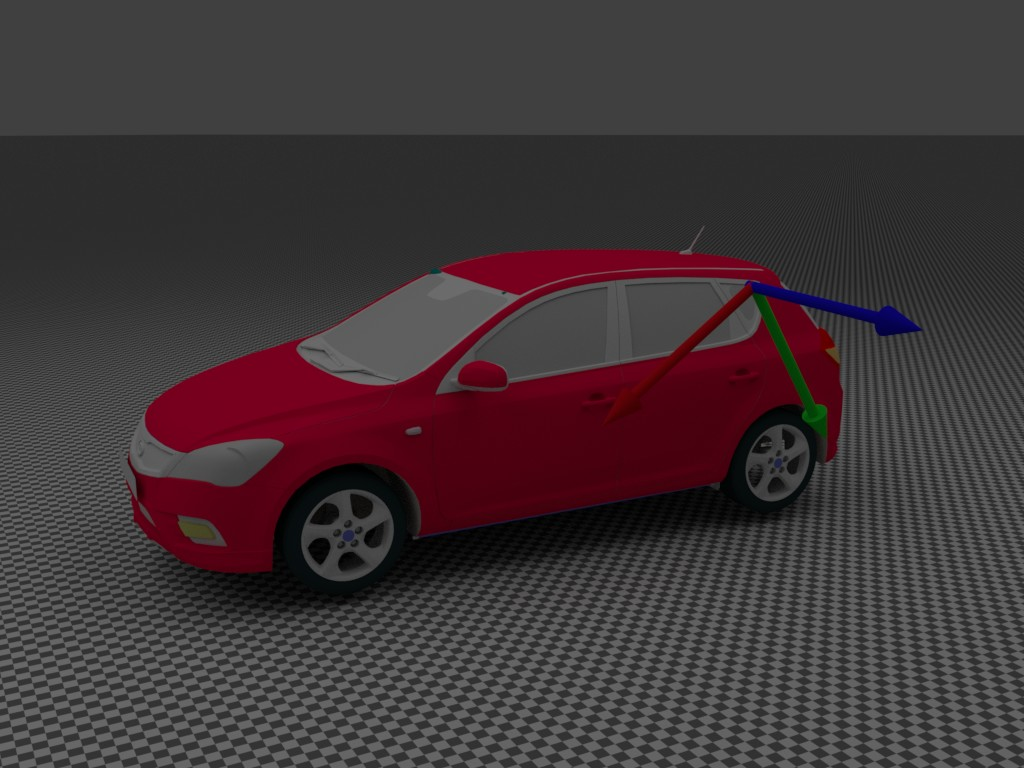
\includegraphics[width=\textwidth]{kia_bad_z_align.jpg}
\caption{Axes shows a sensor bad vertical alignment}
\end{figure}
\justify
Once obtained the rotation angle, the program rotates both local acceleration and angular velocities. After having done that, if in a following stationary time a bad vertical alignment is still found, the program prints a warning on the console to notify that the box become misaligned during motion.

\section{Correction of horizontal alignment}
\begin{figure}[H]
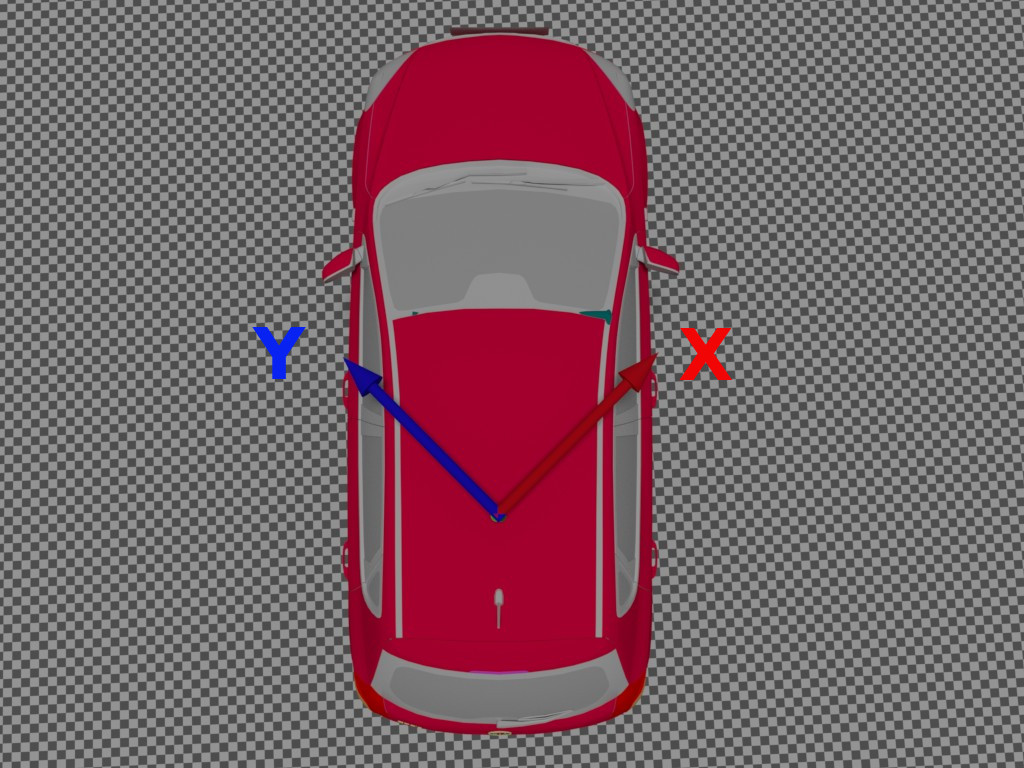
\includegraphics[width=\textwidth]{kia_bad_xy_align.jpg}
\end{figure}
\justify
Box horizontal unalignment is corrected by looking for situations where $a_x>0, \ a_y>0, \omega_z =0$. If this state exists, then or the car is sliding on ice or there is an unalignment on the $xy$ plane. Where, for example, an acceleration forward will be measured with both positive accelerations along x and y axis. 
Still in the situation described, the misalignment can be measured and corrected, still by rotating both local accelerations and angular velocities.

